
% WARNING!  Do not type any of the following 10 characters except as directed:
%                &   $   #   %   _   {   }   ^   ~   \
%
%%
%%  default option for pdfx.sty  if not specified on the command-line.
\providecommand{\pdfxopt}{a-1b}
%%
%%  Use  {filecontents}  for the  .xmpdata file before input encoding is specified.
%%
%%%%%%%%%%%%%%%%%%%%%%%%%%%%%%%%%%%%%%%%%%%%%%%%%%%
\begin{filecontents*}{\jobname.xmpdata}
	% a macro definition, used below
	\pdfxEnableCommands{% simple macro definitions can be provided everything expands to characters
	 \def\RossPete{Ross \& Pete}
	 }
	\Title{Linear Algebra (\jobname)}%  *not* set by LaTeX's  \title
	\Author{Jason Siefken\sep et al.}% *not* set by LaTeX's \author
	\Subject{Linear Algebra textbook/workbook}
	\Keywords{linear algebra\sep vectors\sep mathematics\sep textbook}
	\Org{University of Toronto}
	\CreatorTool{LaTeX + pdfx.sty with options \pdfxopt}
	\Copyright{Jason Siefken}
	\WebStatement{https://github.com/siefkenj/IBLLinearAlgebra/}% should be URL to copyright statement on the web
	\CoverDisplayDate{2019}
	\CoverDate{2019-08-014}%  must be in format  YYYY-MM-DD  or  YYYY-MM
	\Doi{0.0.0.0}%
	%
	% setting the color profile, these reproduce the defaults; use your own, if required
	%
	% RGB is used with PDF/A (4 parameters):
	\setRGBcolorprofile{sRGB_IEC61966-2-1_black_scaled.icc}{sRGB_IEC61966-2-1_black_scaled}{sRGB IEC61966 v2.1 with black scaling}{http://www.color.org}
	%
	%  For Adobe Color Profiles, set the directory for your system
	%
	%  e.g.  on Mac OS X
	%  What is it under Windows ?
	%
	\gdef\ColorProfileDir{./common/}
	% 
	%  For available profiles, see file  AdobeColorProfiles.tex
	%  For PDF/X-4p or PDF/X-5pg   see file  AdobeExternalProfiles.tex
	%
	%  Now you can use the macros defined in those files:
	 \FOGRAXXXIX
	%
	% or CMYK is used with  PDF/X (4 parameters)
	% \setCMYKcolorprofile{\ColorProfileDir coated_FOGRA39L_argl.icc}{Coated FOGRA39}{FOGRA39 (ISO Coated v2 300\%\space (ECI))}{http://www.color.org}
\end{filecontents*}

\documentclass{workbook}


% pdfx will set color profile etc. information appropriately, so the pdf renders
% consistently across devices. But, it doesn't work with the xelatex-based tectonics
\usepackage{ifxetex}
	\usepackage[utf8]{inputenc}
\ifxetex
\else
	\usepackage[a-3u]{pdfx}
\fi

%%%
% import all needed packages and macros
%%%
\usepackage[yyyymmdd]{datetime}
%%
%% All packages and macros needed for the problemsets
%%

\usepackage{amsmath}

\usepackage{lipsum}
%\usepackage{showframe}
%\usepackage{layout}


\usepackage[charter,cal=cmcal]{mathdesign} %different font
%\usepackage{avant}

\usepackage{microtype}
\usepackage{mathtools}
\usepackage{etoolbox}
%\usepackage{amsfonts}
%\usepackage{amssymb}
\usepackage{graphicx}
\graphicspath{{images/}}
\usepackage[inline]{enumitem}
\usepackage{xparse}
\usepackage{ifthen}
\usepackage{caption}
\usepackage{subcaption}
\usepackage{tikz}
	\usetikzlibrary{fit}
	\usetikzlibrary{fadings}
	\usetikzlibrary{calc}
	\tikzset{>=latex}
	\usetikzlibrary{cd}
	\usetikzlibrary{spy}
	\usetikzlibrary{patterns}
	\usetikzlibrary{decorations, decorations.pathreplacing, decorations.markings}

\usepackage{fancyhdr}
\usepackage{calc}
\usepackage{wrapfig}
\usepackage{marginnote}
\usepackage{mparhack}
\usepackage{marginfix}
\usepackage{indextools}
\usepackage[open=false]{bookmark}  % render the pdf TOC in the proper order
\hypersetup{
	hidelinks=true,
	linkcolor = {0 0 1},
	unicode=true,
	psdextra=true,
}
\usepackage{common/nicematrix}

%\usepackage[
%  linktocpage=false,      % no page numbers are clickable
%  colorlinks=false,       % no color
%  breaklinks=true,        % break URLs
%  bookmarks,              % creates bookmarks in pdf
%  hyperfootnotes=true,    % clickable footnotes
%  pdfborder={0 0 0},      % for removing borders around links
%  bookmarksnumbered=true, % If Acrobat bookmarks are requested, include section numbers.
%  bookmarksopen=false,    % If Acrobat bookmarks are requested, show them with all the subtrees expanded.
%  %hidelinks=true,
%  %linkcolor=blue,
%  %citecolor=blue,
%  %urlcolor=blue,
%  pdfpagemode={UseOutlines}, % show pdf bookmarks (indices) on startup; does not function all the time
%  pdftitle={...}, % title
%  pdfauthor={...}, % author
%  pdfkeywords={...}, % subject of the document
%  pdfsubject={...}, % list of keywords
%  pdfmenubar=true,        % make PDF viewer’s menu bar visible
%  pdfpagelabels,
%]{hyperref}
%\usepackage[hidelinks,]{hyperref}
\usepackage{fnpct} % fancy footnote spacing
\usepackage{bm}
\usepackage{systeme}
\usepackage{datatool}% http://ctan.org/pkg/datatool for sorted lists
\usepackage{xspace}


\usepackage{pgfplots}
\pgfplotsset{compat=1.16}
	\usepgfplotslibrary{fillbetween}
%%%
% Useful Linear Algebra macros
%%%
\newcommand{\declarecommand}[1]{\providecommand{#1}{}\renewcommand{#1}}
\DeclareDocumentCommand{\R}{}{\mathbb{R}}  % we don't care if it's already defined.  We really want *this* command!
\DeclareDocumentCommand{\Z}{}{\mathbb{Z}}
\DeclareDocumentCommand{\Q}{}{\mathbb{Q}}
\DeclareDocumentCommand{\N}{}{\mathbb{N}}
\DeclareDocumentCommand{\C}{}{\mathbb{C}}
\DeclareDocumentCommand{\d}{}{\mathrm{d}}
\DeclareDocumentCommand{\dd}{}{\mathbbm{d}} % exterior derivative
\DeclareMathOperator{\Span}{span}
\DeclareMathOperator{\Img}{img}
\DeclareMathOperator{\Id}{id}
\DeclareMathOperator{\Ident}{\Id}
\DeclareMathOperator{\Vol}{Vol}
\DeclareMathOperator{\VolChange}{Vol\hspace{1.5pt}Change}
\DeclareMathOperator{\Range}{range}
\DeclareMathOperator{\Rref}{rref}
\DeclareMathOperator{\Rank}{rank}
\DeclareMathOperator{\Comp}{\Vcomp}
\DeclareMathOperator{\Vcomp}{v\hspace{1pt}comp}
\DeclareMathOperator{\Null}{null}
\DeclareMathOperator{\Nullity}{nullity}
\DeclareMathOperator{\Char}{char}
\DeclareMathOperator{\Proj}{proj}
\DeclareMathOperator{\Flux}{Flux}
\DeclareMathOperator{\Circ}{Circ}
\DeclareMathOperator{\chr}{char}
\DeclareMathOperator{\Dim}{dim}
\DeclareMathOperator{\Perp}{perp}
\DeclareMathOperator{\Ker}{kernel}
\DeclareMathOperator{\Row}{row}
\DeclareMathOperator{\Col}{col}
\DeclareMathOperator{\Rep}{Rep}
\newcommand{\BasisChange}[2]{[#2\!\leftarrow\!#1]}
\newcommand{\proj}{\Proj}
\newcommand{\rref}{\Rref}
\newcommand{\xhat}{{\vec e_1}}
\newcommand{\yhat}{{\vec e_2}}
\newcommand{\zhat}{{\vec e_3}}
\newcommand{\sbasis}[1]{\vec { e}_{#1}}
\newcommand{\mat}[1]{\begin{bmatrix*}[r]#1\end{bmatrix*}}
\newcommand{\matc}[1]{\begin{bmatrix}#1\end{bmatrix}}
\newcommand{\formarg}[2]{\big(#1;\, #2\big)}
\DeclarePairedDelimiter\abs{\lvert}{\rvert}
\DeclarePairedDelimiter\Abs{\lvert}{\rvert}
\DeclarePairedDelimiter\norm{\lVert}{\rVert}
\newcommand{\Norm}[1]{\norm{#1}}
% just to make sure it exists
\providecommand\given{}
% can be useful to refer to this outside \Set
\newcommand\SetSymbol[1][]{%
	\nonscript\::%
	\allowbreak
	\nonscript\:
	\mathopen{}}
\DeclarePairedDelimiterX\Set[1]\{\}{%
	\renewcommand\given{\SetSymbol[\delimsize]}
	#1
}
\newcommand{\Rrefto}{\xrightarrow{\text{row reduces to}}}


% redefine bmatrix,etc to allow optional argument for augmenting
% code from https://tex.stackexchange.com/questions/2233/whats-the-best-way-make-an-augmented-coefficient-matrix
\makeatletter
\renewcommand*\env@matrix[1][*\c@MaxMatrixCols c]{%
  \hskip -\arraycolsep
  \let\@ifnextchar\new@ifnextchar
  \array{#1}}
\makeatother

\newcommand{\scaledgrid}[1]{%
	\begin{tikzpicture}[scale=#1]
		\draw[thin, white!20!black, dotted] (-4.1,-4.1) grid (4.1,4.1);
		\draw[ <->] (-4.3,0) -- (4.3,0);
		\draw[ <->] (0,-4.3) -- (0,4.3);
	\end{tikzpicture}
}
\newcommand{\scaledshortgrid}[1]{%
	\begin{tikzpicture}[scale=#1]
		\draw[thin, white!20!black, dotted] (-4.1,-2.1) grid (4.1,2.1);
		\draw[ <->] (-4.3,0) -- (4.3,0);
		\draw[ <->] (0,-2.3) -- (0,2.3);
	\end{tikzpicture}
}
\newcommand{\singlegrid}{\scaledgrid{1}}
\newcommand{\doublegrid}{\mbox{\scaledgrid{.9}\scaledgrid{.9}}\par}
\newcommand{\triplegrid}{\mbox{\scaledgrid{.6}\scaledgrid{.6}\scaledgrid{.6}}\par}

% labels for source attributions
\NewDocumentCommand{\beezer}{o}{%
	\IfNoValueTF{#1}{%
		{\color{blue}\sffamily{B}}%
	}{%
		{\color{blue}\sffamily{B}}%  XXX Todo, make this href to the appropriate problem number
	}\xspace%
}
\NewDocumentCommand{\hefferon}{o}{%
	\IfNoValueTF{#1}{%
		{\color{blue}\sffamily{H}}%
	}{%
		{\color{blue}\sffamily{H}}%  XXX Todo, make this href to the appropriate problem number
	}\xspace%
}

\DeclareDocumentEnvironment{beforeyouread}{}{
Before you read, make sure you are comfortable with the following.
Please do the ``Quick Check'' problem to see if you are comfortable with each
task.
\begin{itemize}
}{
\end{itemize}
}
\newcommand\quickcheck[1]{\par {\footnotesize \textsc{Quick Check.} \textrm{#1}}}

% Dummy, voidable environments
\DeclareDocumentEnvironment{bookonly}{o}{}{}
\DeclareDocumentEnvironment{displayonly}{o}{}{}


% in non-xelatex engines, hyperref is loaded by `pdfx`. If `pdfx` is not loaded, load it here.
\ifxetex
	\usepackage{hyperref}
\else
\fi

%%%
% Set up the footers to have the correct copyright notices
%%%

\fancypagestyle{siefken}{%
	\rfoot{\footnotesize\it \copyright\,Jason Siefken, 2015--2019 \ \makebox(30,5){
\includegraphics[height=1.2em]{by-sa.pdf}}}
	\lfoot{}
	\renewcommand{\headrulewidth}{0pt}
}
\fancypagestyle{iola}{%
	\rfoot{\footnotesize\it \copyright\,IOLA Team \url{iola.math.vt.edu} \ \makebox(30,5){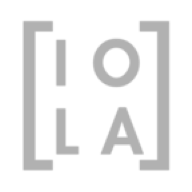
\includegraphics[height=2.2em]{images/iolalogo.png}}}
	\lfoot{}
	\renewcommand{\headrulewidth}{0pt}
}

\DeclareDocumentEnvironment{iola}{o}{%
	\newpage
	\pagestyle{iola}
}{%
	\newpage
}


%%
% Allow hiding of environments
%%
\usepackage{environ}% http://ctan.org/pkg/environ
\makeatletter
\newcommand{\voidenvironment}[1]{%
  \expandafter\providecommand\csname env@#1@save@env\endcsname{}%
  \expandafter\providecommand\csname env@#1@process\endcsname{}%
  \@ifundefined{#1}{}{\RenewEnviron{#1}{}}%
}
\makeatother
% allow pagebreaks that only display in `standard` mode
\newcommand{\displayonlynewpage}{\begin{displayonly}\newpage\end{displayonly}}
% allow pagebreaks that only display in `book` mode
\newcommand{\bookonlynewpage}{\begin{bookonly}\newpage\end{bookonly}}




\setbookoptions{
	twosided = false,
	inline solutions = false,
}


\NewColoredEnvironment{
	name = lesson,
	display name = Lesson,
	banner color = Plum,
	title color = Plum,
	banner on left = true,
	open right = false,
}
\NewColoredEnvironment{
	name = module,
	display name = Module,
	banner color = Turquoise,
	title color = Cerulean,
	definition color = Cerulean,
	theorem color = myorange,
}
\NewColoredEnvironment{
	name = appendix,
	display name = Appendix,
	banner color = Green,
}


\voidenvironment{solution}
\voidenvironment{bookonly}
\voidenvironment{annotation}
\voidenvironment{lesson}
\voidenvironment{module}

\makeatletter
\ExplSyntaxOn
\_workbook_define_new_theorem_box:nn {definition} {
	% For definitions, we just print the term being defined without the word "Definition" in front.
	display~name = {},
	color = LimeGreen,
	bgcolor = LimeGreen!10!white,
}

\DeclareDocumentCommand{\SlideTitle}{o}{
	\textbf{\sffamily
		Core~Exercise~\int_eval:n {\thequestion + (\IfNoValueTF{#1}{0}{#1})}
	}
}
\DeclareDocumentCommand{\TypesetSlideFooter}{m}{
	\dim_set:Nn \l_tmpa_dim {#1}
	\begin{tikzpicture}[remember~picture, overlay]
		\fill[cyan!50!black] ($(current~page.south~west) + (0,\l_tmpa_dim)$) rectangle (current~page.south~east);
	\end{tikzpicture}
}
\DeclareDocumentCommand{\TypsetSlideHeader}{o m}{
	\dim_set:Nn \l_tmpa_dim {#2}
	\begin{tikzpicture}[remember~picture, overlay]
		\draw[fill=cyan!50!black] ($(current~page.north~west) + (0,-\l_tmpa_dim)$) rectangle (current~page.north~east) 
			node[pos=0, anchor=west, color=white, xshift=1ex, yshift=.5\l_tmpa_dim]{\SlideTitle[#1]};
	\end{tikzpicture}
}

\box_new:N \g_workbook_slide_body_box
\box_new:N \l_workbook_slide_body_tmp_box
\dim_new:N \g_workbook_slide_bodyvailable_height_dim
\dim_new:N \l_workbook_slide_body_request_height_dim
\dim_new:N \l_workbook_slide_body_request_multicol_height_dim
\dim_new:N \l_workbook_slide_minipage_width_dim
\newcounter{question_at_start}
% Typeset to a box. The first arg is the question number to start at
% followed by a font-adjustment command, followed by the material to be typeset
\DeclareDocumentCommand{\TypesetSlideBodyOneCol}{m m +m}{
	\vbox_gset:Nn \g_workbook_slide_body_box {
		\setcounter{question}{#1}
		#2
		\setlength{\fboxrule}{0pt} 
		\fbox{
			\begin{minipage}{\l_workbook_slide_minipage_width_dim}
				#3
			\end{minipage}
		}
	}
}
\DeclareDocumentCommand{\TypesetSlideBodyTwoCol}{m m +m}{
	\vbox_gset:Nn \g_workbook_slide_body_box {
		% We're re-typesetting to see if we can get a better fit. Reset the question counter
		% before this.
		\setcounter{question}{#1}
		% A (possibly blank) font-adjustment command, like \small
		#2
		\setlength{\fboxrule}{0pt} 
		\fbox{
			\begin{minipage}{\l_workbook_slide_minipage_width_dim}
				\begin{multicols}{2}
					#3
				\end{multicols}
			\end{minipage}
		}
	}
}
% Attempt to typeset the slide body as one column or two columns
% choosing the layout that achieves the "best fit" (i.e., needs the least
% amount to scaling).
\dim_new:N \g_workbook_slide_body_request_height
\DeclareDocumentCommand{\TypesetSlideBodyBestFit}{m m m +m}{
	\dim_set:Nn \g_workbook_slide_bodyvailable_height_dim {#1}
	\def\questionStartNumber{#2}
	\def\fontCommand{#3}

	% Try to typeset in one column
	\TypesetSlideBodyOneCol{\questionStartNumber}{\fontCommand}{#4}
	\dim_set:Nn \l_workbook_slide_body_request_height_dim {\box_ht:N \g_workbook_slide_body_box + \box_dp:N \g_workbook_slide_body_box}
	\dim_gset_eq:NN \g_workbook_slide_body_request_height \l_workbook_slide_body_request_height_dim
	
	% If we're too tall, try to typeset as two columns
	\dim_compare:nNnTF {\l_workbook_slide_body_request_height_dim} > {\g_workbook_slide_bodyvailable_height_dim} {
		% scale the original contents so that it fits
		\box_gresize_to_ht_plus_dp:Nn \g_workbook_slide_body_box {\g_workbook_slide_bodyvailable_height_dim}
		\box_gset_eq:NN \l_workbook_slide_body_tmp_box \g_workbook_slide_body_box

		% Try typesetting as two columns
		\TypesetSlideBodyTwoCol{\questionStartNumber}{\fontCommand}{#4}

		% The two-column render might also be too tall; resize if needed
		\dim_set:Nn \l_workbook_slide_body_request_multicol_height_dim {\box_ht:N \g_workbook_slide_body_box + \box_dp:N \g_workbook_slide_body_box}
		\dim_compare:nNnTF {\l_workbook_slide_body_request_multicol_height_dim} > {\g_workbook_slide_bodyvailable_height_dim} {
			\box_gresize_to_ht_plus_dp:Nn \g_workbook_slide_body_box {\g_workbook_slide_bodyvailable_height_dim}
		}{}

		% Pick the better fit and assign it to box a.
		\dim_compare:nNnTF {\l_workbook_slide_body_request_multicol_height_dim} > {\l_workbook_slide_body_request_height_dim} {
			\box_gset_eq:NN \g_workbook_slide_body_box \l_workbook_slide_body_tmp_box
		}{
			\dim_gset_eq:NN \g_workbook_slide_body_request_height \l_workbook_slide_body_request_multicol_height_dim
		}
	}{}
}

% Typeset the slide body. Arguments 1 and 2 are the top and bottom margins
\DeclareDocumentCommand{\TypesetSlideBody}{m m +m}{
	\dim_set:Nn \g_workbook_slide_bodyvailable_height_dim {10cm - (#1) - (#2)}
	\dim_set:Nn \l_workbook_slide_minipage_width_dim {\linewidth - .35cm}
	\box_clear:N \g_workbook_slide_body_box
	\box_clear:N \l_workbook_slide_body_tmp_box
	\setcounter{question_at_start}{\thequestion}

	% Try to typeset in a normal font size
	\TypesetSlideBodyBestFit{\g_workbook_slide_bodyvailable_height_dim}{\thequestion_at_start}{}{#3}
	% If we're too tall by a little bit, we just use the scaled result.
	% Otherwise we will try typesetting with a smaller font.
	% Since the height of a slide is 10cm, we can use 1cm as 10%, etc.
	\dim_compare:nNnTF {\g_workbook_slide_body_request_height - \g_workbook_slide_bodyvailable_height_dim} < {1cm} {}{
		\TypesetSlideBodyBestFit{\g_workbook_slide_bodyvailable_height_dim}{\thequestion_at_start}{\small}{#3}
		\dim_compare:nNnTF {\g_workbook_slide_body_request_height - \g_workbook_slide_bodyvailable_height_dim} < {1cm} {}{
			\TypesetSlideBodyBestFit{\g_workbook_slide_bodyvailable_height_dim}{\thequestion_at_start}{\footnotesize}{#3}
		}
	}
}

\prop_new:N \g_workbook_slide_info_prop
\dim_new:N \_workbook_current_parskip
\prop_put:Nnn \g_workbook_slide_info_prop {last_page} {0}
\prop_put:Nnn \g_workbook_slide_info_prop {margin_top} {.6cm}
\prop_put:Nnn \g_workbook_slide_info_prop {margin_bottom} {3cm}

% Slide environment. It's contents are typeset as one or two columns, depending on what fits on the
% page better. The optional argument is a number 
\DeclareDocumentEnvironment{slide}{o +b}{
	% We typeset everything in a minipage, so we need to remember the parskip.
	\dim_set_eq:NN \_workbook_current_parskip \parskip

	% The \question macro shouldn't do anything other than increment the question counter.
	% We typeset the question number manually
	\DeclareDocumentCommand{\question}{}{
		\addtocounter{question}{1}
		\def\@currentlabel{\thequestion}
	}

	\clearpage
	% Determine if we need a manual page break based on whether the previous slide was printed
	% on the same page.
	\prop_put:Nnx \g_workbook_slide_info_prop {curr_page} {\thepage}
	\int_compare:nNnTF {\prop_item:Nn \g_workbook_slide_info_prop {curr_page}} = {\prop_item:Nn \g_workbook_slide_info_prop {last_page}} {
		\clearpage
	} {}
	\prop_put:Nnx \g_workbook_slide_info_prop {curr_page} {\thepage}

	% Save the question number from the start and end of the slide so we can
	% compute how many questions are contained in this slide.
	\prop_put:Nnx \g_workbook_slide_info_prop {question_at_start} {\thequestion}
	\TypesetSlideBody{
		\prop_item:Nn \g_workbook_slide_info_prop {margin_top}
	}{
		\prop_item:Nn \g_workbook_slide_info_prop {margin_bottom}
	}{
		#2
	}
	\prop_put:Nnx \g_workbook_slide_info_prop {question_at_end} {\thequestion}
	\prop_put:Nnx \g_workbook_slide_info_prop {num_questions} {
		\int_eval:n {\prop_item:Nn \g_workbook_slide_info_prop {question_at_end} - \prop_item:Nn \g_workbook_slide_info_prop {question_at_start}}
	}

	% Footer
	\TypesetSlideFooter{\prop_item:Nn \g_workbook_slide_info_prop {margin_bottom}}
	% Header
	\TypsetSlideHeader[#1]{\prop_item:Nn \g_workbook_slide_info_prop {margin_top}}
	% Body (typeset last so it appears on top of the header and footer for any overflows.
	% It is centered in case it has been scaled to fit.
	\hfil\box_use:N \g_workbook_slide_body_box\hfil

}{}


\DeclareDocumentEnvironment{parts}{o +b}{
	\nopagebreak
	\begin{list}{\formatpartsitem}{
			\usecounter{partsitem}
			\setlength{\leftmargin}{.6cm}
			\setlength{\itemsep}{0cm}
			\setlength{\topsep}{0cm}
		}
		% if we gave the [resume] argument, start counting from where we
		% left off.
		\ifthenelse{ \equal{#1}{resume} }{
			\setcounter{partsitem}{\value{partsitemlast}}
		}{}
	
		% we'd like an sub-enumerate environments
		% to act like they're nested, so advance
		% the level by one.
		\advance\@enumdepth\@ne
		#2
		\setcounter{partsitemlast}{\value{partsitem}}
	\end{list}
}{
}
\RenewDocumentCommand{\section}{sm}{}
\RenewDocumentCommand{\subsection}{sm}{}


% Set the geometry appropriately
\geometry{
	%papersize={13.3cm, 10cm},
	papersize={17.7cm, 10cm},
	twoside=false,
	noheadfoot,
	marginpar=0pt,
	marginparsep=0pt,
	includeall,
	left=0cm,
	right=0cm,
	top=.7cm,
	bottom=.7cm,
	%showframe
}
\geometry{bottom=\dim_eval:n {\prop_item:Nn \g_workbook_slide_info_prop {margin_bottom}}}
\geometry{top=\dim_eval:n {\prop_item:Nn \g_workbook_slide_info_prop {margin_top}}}



\ExplSyntaxOff
\makeatother



\begin{document}
%%
%% Import definitions from definition.tex; all definitions can be restated multiple times
%%

%%
%% Start Definitions (each of these we can reuse)
%%
\begin{SaveDefinition}[
		key=SubsetSuperset,
		title={Subset \& Superset}
	]
	The set $B$ is a \emph{subset}\index[definitions]{Subset} of the set $A$, written $B\subseteq A$\index[symbols]{$\subseteq$}, if for all
	$b\in B$ we also have $b\in A$.  In this case, $A$ is called a \emph{superset}\index[definitions]{Superset}
	of $B$.\footnote{
		Some mathematicians use the symbol $\subset$ instead of $\subseteq$.}
\end{SaveDefinition}
\begin{SaveDefinition}[
		key=SetEquality,
		title={Set Equality}
	]
	The sets $A$ and $B$ are \emph{equal}\index{Set!equality}\index[definitions]{Set!equality}, written $A=B$, if $A\subseteq B$ and $B\subseteq A$.
\end{SaveDefinition}
\begin{SaveDefinition}[
		key=SetSubtraction,
		title={Set Subtraction}
	]
	For sets $A$ and $B$, the \emph{set-wise difference}\index[definitions]{Set!subtraction}\index{Set!subtraction} between $A$ and $B$,
	written $A\backslash B$, is the set
	\[
		A\backslash B = \Set{x\given x\in A\text{ and }x\notin B}.
	\]
\end{SaveDefinition}
\begin{SaveDefinition}[
		key=UnionsIntersections,
		title={Unions \& Intersections}
	]
	Let $X$ and $Y$ be sets. The \emph{union}\index[definitions]{Set!union}\index{Set!union}\index[symbols]{$\cup$} of $X$ and $Y$ and the
	\emph{intersection}\index[definitions]{Set!intersection}\index{Set!intersection}\index[symbols]{$\cap$} of $X$
	and $Y$ are defined as follows.

	\smallskip

	\hfill\begin{minipage}{\dimexpr\textwidth-3cm}
	\begin{itemize}
		\item[(union)] $X\cup Y = \Set{ a \given a\in X\text{ or }a\in Y}$.
		\item[(intersection)] $X\cap Y = \Set{ a \given a\in X\text{ and }a\in Y}$.
	\end{itemize}
	\end{minipage}
\end{SaveDefinition}

\begin{SaveDefinition}[key=Set, title={Set}]
	A \emph{set}\index[definitions]{Set} is a (possibly infinite) collection of items and is notated
	with curly braces (for example, $\{1,2,3\}$ is the set containing the
	numbers 1, 2, and 3). We call the items in a set
	\emph{elements}.

	If $X$ is a set and $a$ is an element of $X$, we may write $a\in X$,
	which is read ``$a$ is an element of $X$.''

	If $X$ is a set, a
	\emph{subset} $Y$ of $X$ (written $Y\subseteq X$) is a set such that
	every element of $Y$ is an element of $X$. Two sets are called
	\emph{equal} if they are subsets of each other (i.e., $X=Y$ if $X\subseteq
	Y$ and $Y\subseteq X$).

	We can define a subset using
	\emph{set-builder notation}. That is, if $X$ is a set, we can define the
	subset
	\[
		Y= \Set*{a\in X \given \text{some rule involving }a},
	\]
	 which is read ``$Y$ is the set of $a$ in $X$ {\bf such that} some rule
	involving $a$ is true.'' If $X$ is intuitive, we may omit it and simply write
	$Y=\{a:\text{some rule involving }a\}$. You may equivalently use ``$|$''
	instead of ``$:$'', writing $Y=\{a\,|\,\text{some rule involving }a\}$.
\end{SaveDefinition}

\begin{SaveDefinition}[key=ZeroVector, title={Zero Vector}]
		The \emph{zero vector}\index{Zero vector ($\vec 0$)}\index[definitions]{Zero vector ($\vec 0$)}, notated as $\vec 0$\index[symbols]{$\vec 0$},
		is the vector with no magnitude.
\end{SaveDefinition}

\begin{SaveDefinition}[key=LinearCombination, title={Linear Combination}]
	A \emph{linear combination}\index{Linear combination}\index[definitions]{Linear combination} of the vectors
	$\vec v_{1},\vec v_{2},\ldots,\vec v_{n}$ is a vector
	\[
		\vec w = \alpha_{1}\vec v_{1}+\alpha_{2}\vec v_{2}+\cdots+\alpha_{n}\vec
		v_{n}.
	\]
	 The scalars $\alpha_{1},\alpha_{2},\ldots,\alpha_{n}$ are called the
	\emph{coefficients}\index{Linear combination!coefficient of}\index[definitions]{Linear combination!coefficient of} of the linear combination.
\end{SaveDefinition}

\begin{SaveDefinition}[
	key=NonnegativeConvexLinearCombinations,
	title={Non-negative \& Convex Linear Combinations}]

	Let
	$\vec w=\alpha_{1}\vec v_{1}+\alpha_{2}\vec v_{2}+\cdots+\alpha_{n}\vec
	v_{n}.$
	The vector $\vec w$ is called a
	\emph{non-negative}\index{Linear combination!non-negative}\index[definitions]{Linear combination!non-negative} linear combination of
	$\vec v_{1},\vec v_{2},\ldots,\vec v_{n}$ if
	\[\alpha_{1},\alpha_{2},\ldots,\alpha_{n}\geq 0.\]

	The vector $\vec w$ is called a
	\emph{convex}\index{Linear combination!convex}\index[definitions]{Linear combination!convex} linear combination of
	$\vec v_{1},\vec v_{2},\ldots,\vec v_{n}$
	if \[\alpha_{1},\alpha_{2},\ldots,\alpha_{n}\geq 0\qquad\text{and}\qquad
	\alpha_{1}+\alpha_{2}+\cdots+\alpha_{n}=1.\]
\end{SaveDefinition}

\begin{SaveDefinition}[key=VectorFormofaLine, title={Vector Form of a Line}]
	Let $\ell$ be a line and let $\vec d$ and $\vec p$ be vectors. If $\ell=\Set{\vec
	x\given \vec x= t\vec d+\vec p\text{ for some } t\in\R }$, we say the vector equation

	\[
		\vec x=t\vec d+\vec p
	\]
	 is $\ell$ expressed in
	\emph{vector form}\index{Line!vector form of}\index[definitions]{Line!vector form of}. The vector $\vec d$ is called a
	\emph{direction vector}\index{Line!direction vector for}\index[definitions]{Line!direction vector for} for $\ell$.
\end{SaveDefinition}

\begin{SaveDefinition}[key=VectorFormofaPlane, title={Vector Form of a Plane}]
	A plane $\mathcal P$ is written in
	\emph{vector form}\index{Plane!vector form of}\index[definitions]{Plane!vector form of} if it is expressed as
	\[
		\vec x=t\vec d_{1} +s\vec d_{2}+\vec p
	\]
	 for some vectors $\vec d_{1}$ and $\vec d_{2}$ and point $\vec p$. That
	is,
	$\mathcal P = \{\vec x: \vec x= t\vec d_{1}+s\vec d_{2} +\vec p\text{ for
	some }t,s\in\R \}$. The vectors $\vec d_{1}$ and $\vec d_{2}$ are called
	\emph{direction vectors}\index{Plane!direction vector for}\index[definitions]{Plane!direction vector for} for $\mathcal P$.
\end{SaveDefinition}

\begin{SaveDefinition}[key=Span, title={Span}]
	The
	\emph{span}\index{Span}\index[definitions]{Span} of a set of vectors $V$ is the set of all linear
	combinations of vectors in $V$. That is,
	\begin{dmath*}
		\Span V = \Set{{\vec v \given \vec v=}\,\alpha_1\vec v_1+\alpha_2\vec
		v_2 + \cdots +\alpha_n\vec v_n \allowbreak \text{ for some } \allowbreak {\vec v_1,\vec v_2,\ldots,\vec
		v_n\in V}\! \text{ and scalars }\alpha_1,\alpha_2,\ldots,\alpha_n}.
	\end{dmath*}
	\index[symbols]{$\Span V$}

	Additionally, we define $\Span\Set{} = \Set{\vec 0}$.
\end{SaveDefinition}

\begin{SaveDefinition}[key=SetAddition, title={Set Addition}]
	If $A$ and $B$ are sets of vectors, then the
	\emph{set sum}\index{Set sum}\index[definitions]{Set sum} of $A$ and $B$, denoted $A+B$, is
	\[
		A+B=\Set{\vec x \given \vec x=\vec a+\vec b\text{ for some }\vec
		a\in A\text{ and } \vec b\in B}.
	\]

\end{SaveDefinition}

\begin{SaveDefinition}[
	key=LinearlyDependentIndependentGeometric,
	title={Linearly Dependent \& Independent (Geometric)}]

	We say the vectors $\vec v_{1},\vec v_{2},\ldots,\vec v_{n}$ are
	\emph{linearly dependent}\index{Linearly dependent} if for at least one $i$,
	\[
		\vec v_{i}\in\Span\Set{\vec v_1,\vec v_2,\ldots,\vec v_{i-1}, \vec
		v_{i+1},\ldots,\vec v_n}.
	\]
	 Otherwise, they are called
	\emph{linearly independent}\index{Linearly independent}\index[definitions]{Linear dependence/independence!geometric definition}.
\end{SaveDefinition}

\begin{SaveDefinition}[
	key=TrivialLinearCombination,
	title={Trivial Linear Combination}]

	The linear combination $\alpha_1\vec v_1+\cdots+\alpha_n\vec v_n$ is called
	\emph{trivial}\index{Linear combination!trivial}\index[definitions]{Linear combination!trivial}
	if $\alpha_1=\cdots=\alpha_n=0$. If at least one $\alpha_i\neq 0$,
	the linear combination is called \emph{non-trivial}.
\end{SaveDefinition}

\begin{SaveDefinition}[
	key=LinearlyDependentIndependentAlgebraic,
	title={Linearly Dependent \& Independent (Algebraic)}]

	The vectors $\vec v_{1},\vec v_{2},\ldots,\vec v_{n}$ are
	\emph{linearly dependent} if there is a non-trivial linear combination
	of $\vec v_{1},\ldots,\vec v_{n}$ that equals the zero vector. Otherwise they
	are linearly independent\index[definitions]{Linear dependence/independence!algebraic definition}.
\end{SaveDefinition}

\begin{SaveDefinition}[
	key=HomogeneousSystem,
	title={Homogeneous System}]

	A system of linear equations or a vector equation in the variables $\alpha_1$, \ldots,
	$\alpha_n$ is called
	\emph{homogeneous}\index{System of linear equations!homogeneous}\index[definitions]{Homogeneous system} if it takes the form
	\[
		\alpha_1\vec v_1+\alpha_2\vec v_2+\cdots +\alpha_n\vec v_n=\vec 0,
	\]
	where the right side of the equation is $\vec 0$.
\end{SaveDefinition}


\begin{SaveDefinition}[key=Norm, title={Norm}]
	The
	\emph{norm} of a vector $\vec v=\matc{v_1\\\vdots\\v_n}$ is the length/magnitude
	of $\vec v$. It is written $\|\vec v\|$ and can be computed from the Pythagorean
	formula
	$
		\|\vec v\|=\sqrt{v_1^2+\cdots +v_n^2}.
	$

\end{SaveDefinition}

\begin{SaveDefinition}[key=DotProduct, title={Dot Product}]
	If $\vec a=\matc{a_1\\a_2\\ \vdots\\a_n}$ and
	$\vec b=\matc{b_1\\b_2\\ \vdots\\b_n}$ are two vectors in $n$-dimensional
	space, then the
	\emph{dot product} of $\vec a$ an $\vec b$ is
	\[
		\vec a\cdot\vec b = a_{1}b_{1}+a_{2}b_{2}+\cdots+a_{n}b_{n}.
	\]
	 Equivalently, the dot product is defined by the geometric formula
	\[
		\vec a\cdot \vec b = \|\vec a\|\|\vec b\|\cos \theta
	\]
	 where $\theta$ is the angle between $\vec a$ and $\vec b$.
\end{SaveDefinition}

% There are two choices for this definition: ku=v for some k or u=kv for some k.
% The places where this matters is in the definitions of vector component and
% eigenvector. In particular, for eigenvectors, the informal definition
% "v is a non-zero vector that doesn't change direction" must be understood as
% Av is in the same direction as v (and not the other way around).
\begin{SaveDefinition}[key=Direction, title={Direction}]
	The vector $\vec u$ points in the \emph{direction}\index{Vector!direction of} of
	the vector $\vec v$ if $\vec u=k\vec v$ for some scalar $k$.
	The vector $\vec u$ points in the \emph{positive direction}\index{Vector!positive direction of} of
	$\vec v$ if $\vec u=k\vec v$ for some positive scalar $k$.
\end{SaveDefinition}

\begin{SaveDefinition}[key=Distance, title={Distance}]
	The
	\emph{distance} between two vectors $\vec u$ and $\vec v$ is
	$\|\vec u-\vec v\|$.
\end{SaveDefinition}

\begin{SaveDefinition}[key=UnitVector, title={Unit Vector}]
	A vector $\vec v$ is called a
	\emph{unit vector} if $\|\vec v\|=1$.
\end{SaveDefinition}

\begin{SaveDefinition}[key=Orthogonal, title={Orthogonal}]
	Two vectors $\vec u$ and $\vec v$ are
	\emph{orthogonal}\index{Orthogonal}\index[definitions]{Orthogonal} to each other if $\vec u\cdot \vec v=0$. The word orthogonal
	is synonymous with the word perpendicular.
\end{SaveDefinition}

\begin{SaveDefinition}[key=NormalVector, title={Normal Vector}]
	A
	\emph{normal vector}\index[definitions]{Line!normal vector}\index{Plane!normal vector}\index{Line!normal vector}\index{Plane!normal vector} to a line (or plane or hyperplane) is a non-zero
	vector that is orthogonal to all direction vectors for the line (or plane
	or hyperplane).
\end{SaveDefinition}

\begin{SaveDefinition}[key=NormalFormofaLine, title={Normal Form of a Line}]

	A line $\ell\subseteq \R^2$ is expressed in \emph{normal form}\index[definitions]{Line!normal form}\index{Line!normal form} if there exist
	vectors $\vec n\neq \vec 0$ and $\vec p$ so that $\ell$ is the solution set to the equation
	\[
		\vec n\cdot (\vec x-\vec p)=0.
	\]
	The equation $\vec n\cdot (\vec x-\vec p)=0$ is called the \emph{normal form of $\ell$}.
\end{SaveDefinition}

\begin{SaveDefinition}[key=Hyperplane, title={Hyperplane}]
	The set $X\subseteq \R^n$ is called a \emph{hyperplane}\index{Hyperplane}\index[definitions]{Hyperplane} if there
	exists $\vec n\neq \vec 0$ and $\vec p$ so that $X$ is the set of solutions
	to the equation
	\[
		\vec n\cdot (\vec x-\vec p)=0.
	\]
\end{SaveDefinition}


\begin{SaveDefinition}[key=Projection, title={Projection}]
	Let $X\subseteq \R^n$ be a set. The
	\emph{projection} of the vector $\vec v\in\R^n$ onto $X$, written $\Proj_{X}\vec
	v$, is the closest point in $X$ to $\vec v$.\index[definitions]{Projection}\index{Projection}\index[symbols]{$\Proj_{X}\vec v$}
\end{SaveDefinition}

\begin{SaveDefinition}[key=Component, title={Vector Components}]
	Let $\vec u$ and $\vec v\neq \vec 0$ be vectors. The
	\emph{vector component of $\vec u$ in the $\vec v$ direction}, written $\Comp_{\vec
	v}\vec u$, is the vector in the direction of $\vec v$ so that
	$\vec u-\Comp_{\vec v}\vec u$ is orthogonal to $\vec v$.\index{Vector component}\index[definitions]{Vector component}\index[symbols]{$\Vcomp_{\vec v}\vec u$}
	\begin{center}
		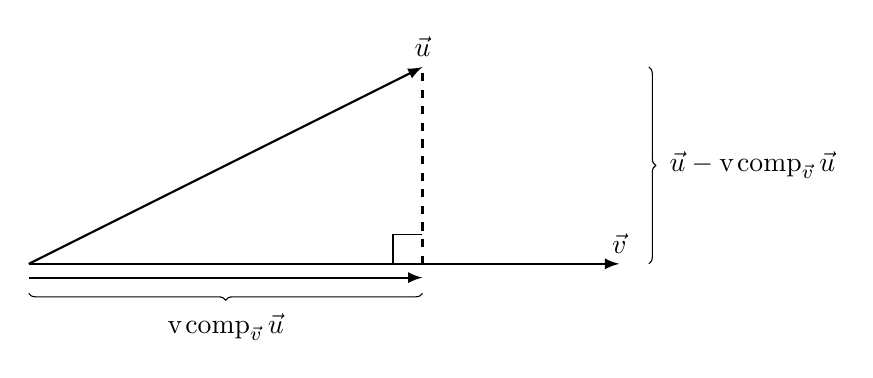
\begin{tikzpicture}[>=latex, scale=2.5]
			\draw[->,thick,black] (0,0) -- (2,1) node [above]
				{$\vec u$};

			\draw[->,thick,black] (0,0) -- (3,0) node [above]
				{$\vec v$};

			\draw[->,thick,black,yshift=-.07cm] (0,0) -- (2,0);
			\draw[decoration={brace, mirror}, decorate, yshift=-.15cm]
				(0,0) -- (2,0) node [midway,below,yshift=-4pt] {$\Comp_{\vec
				v}\vec u$};

			\draw[dashed,thick,black] (2,0) -- (2,1);
			\draw[decoration={brace, mirror}, decorate, xshift=1.15cm]
				(2,0) -- (2,1) node [midway,right,xshift=4pt]
				{$\vec u-\Comp_{\vec v}\vec u$};

			\draw[thin,black] (1.85,0)--(1.85,.15)--(2,.15);
		\end{tikzpicture}
	\end{center}
\end{SaveDefinition}

\begin{SaveDefinition}[key=Subspace, title={Subspace}]
	A non-empty subset $V\subseteq \R^{n}$ is called a \emph{subspace}\index{Subspace}\index[definitions]{Subspaces} if for all $\vec u,\vec v\in V$ and all
	scalars $k$ we have
	\begin{enumerate}
		\item[(i)] $\vec u+\vec v\in V$; and

		\item[(ii)] $k\vec u\in V$.
	\end{enumerate}
\end{SaveDefinition}

\begin{SaveDefinition}[key=TrivialSubspace, title={Trivial Subspace}]
	The subset $\Set{\vec 0}\subseteq\R^n$ is called the \emph{trivial subspace}\index{Subspace!trivial subspace}\index[definitions]{Subspace!trivial subspace}.
\end{SaveDefinition}

\begin{SaveDefinition}[key=Basis, title={Basis}]
	A
	\emph{basis}\index[definitions]{Basis}\index{Basis} for a subspace $\mathcal V$ is a linearly independent set of vectors,
	$\mathcal B$, so that $\Span\mathcal B=\mathcal V$.
\end{SaveDefinition}

\begin{SaveDefinition}[key=Dimension, title={Dimension}]
	The
	\emph{dimension}\index[definitions]{Subspace!dimension}\index{Subspace!dimension} of a subspace $V$ is the number of elements in a basis
	for $V$.
\end{SaveDefinition}

\begin{SaveDefinition}[key=StandardBasisforRn, title={Standard Basis}]
	The \emph{standard basis}\index[definitions]{Basis!standard basis}\index{Basis!standard basis} for $\R^n$ is the set $\Set{\vec e_1,\ldots,\vec e_n}$ where
	\[
		\vec e_1=\matc{1\\0\\0\\\vdots}\qquad
		\vec e_2=\matc{0\\1\\0\\\vdots}\qquad
		\vec e_3=\matc{0\\0\\1\\\vdots}\qquad\cdots.
	\]
	That is $\vec e_i$ is the vector with a $1$ in its
	$i$th coordinate and zeros elsewhere.
\end{SaveDefinition}

\begin{SaveDefinition}[
	key=RepresentationinaBasis,
	title={Representation in a Basis}]

	Let $\mathcal B=\Set{\vec b_1,\ldots,\vec b_n}$ be a basis for a
	subspace $V$ and let $\vec v\in V$. The
	\emph{representation of $\vec v$ in the $\mathcal B$ basis}\index{Vector!representation in a basis}\index[definitions]{Vector!representation in a basis}, notated $[\vec
	v]_{\mathcal B}$\index[symbols]{$[\vec v]_{\mathcal B}$}, is the column matrix
	\[
		[\vec v]_{\mathcal B}= \matc{\alpha_1\\\vdots\\\alpha_n}
	\]
	 where $\alpha_{1},\ldots,\alpha_{n}$ uniquely satisfy
	$\vec v=\alpha_{1}\vec b_{1}+\cdots+\alpha_{n}\vec b_{n}.$

	Conversely,
	\[
		\matc{\alpha_1\\\vdots\\\alpha_n}_{\mathcal B}= \alpha_{1}\vec b_{1}+\cdots
		+\alpha_{n}\vec b_{n}
	\]
	 is notation for the linear combination of $\vec b_{1},\ldots,\vec b_{n}$
	with coefficients $\alpha_{1},\ldots,\alpha_{n}$.
\end{SaveDefinition}

\begin{SaveDefinition}[key=OrthonormalBasis, title={Orthonormal Basis}]
	A basis $\mathcal B=\{\vec b_{1},\ldots,\vec b_{n}\}$ is called
	\emph{orthonormal}\index[definitions]{Basis!orthonormal basis}\index{Basis!orthonormal basis} if every basis vector is a unit vector and all
	basis vectors are orthogonal to each other. That is,
	\[
		\vec b_i\cdot \vec b_j=\begin{cases}
			1 &\text{ if }\quad i=j\\
			0 &\text{ if }\quad i\neq j
		\end{cases}.
	\]
\end{SaveDefinition}

\begin{SaveDefinition}[key=OrientationofaBasis, title={Orientation of a Basis}]
	The ordered basis $\mathcal B=\{\vec b_{1},\ldots,\vec b_{n}\}$ is
	\emph{right-handed}\index[definitions]{Basis!right-handed}\index{Basis!right-handed} or
	\emph{positively oriented}\index[definitions]{Basis!positively oriented}\index{Basis!positively oriented} if it can be continuously transformed to the
	standard basis (with $\vec b_{i}\mapsto \vec e_{i}$) while remaining
	linearly independent throughout the transformation. Otherwise,
	$\mathcal B$ is called
	\emph{left-handed}\index[definitions]{Basis!left-handed}\index{Basis!left-handed} or
	\emph{negatively oriented}\index[definitions]{Basis!negatively oriented}\index{Basis!negatively oriented}.
\end{SaveDefinition}

\begin{SaveDefinition}[key=LinearTransformation, title={Linear Transformation}]
	Let $V$ and $W$ be subspaces. A function $T:V\to W$ is called a
	\emph{linear transformation}\index[definitions]{Linear transformation}\index{Linear transformation} if
	\[
		T(\vec u+\vec v)=T(\vec u)+T(\vec v) \qquad\text{and}\qquad T(\alpha
		\vec v)=\alpha T(\vec v)
	\]
	 for all vectors $\vec u,\vec v\in V$ and all scalars $\alpha$.
\end{SaveDefinition}

\begin{SaveDefinition}[key=ImageofaSet, title={Image of a Set}]
	Let $L:\R^n\to \R^m$ be a transformation and let $X\subseteq \R^n$ be a set. The
	\emph{image of the set $X$ under $L$}\index[definitions]{Set!image of}\index{Set!image of}, denoted $L(X)$\index[symbols]{$L(X)$ (Image of a set)}, is the set
	\[
		L(X)=\Set{\vec y\in \R^m \given \vec y=L(\vec x)\text{ for some }\vec
		x\in X}.
	\]
\end{SaveDefinition}

\begin{SaveDefinition}[key=CompositionofFunctions, title={Composition of Functions}]
	Let $f:A\to B$ and $g:B\to C$. The \emph{composition}\index[definitions]{Function!composition}\index{Function!composition} of $g$ and $f$, notated $g\circ f$\index[symbols]{$g\circ f$},
	is the function $h:A\to C$ defined by
	\[
		h(x)=g\circ f(x) = g\Big(f(x)\Big).
	\]
\end{SaveDefinition}

\begin{SaveDefinition}[key=Range, title={Range}]
	The
	\emph{range} (or
	\emph{image})\index[definitions]{Linear transformation!range (image)}\index{Linear transformation!range (image)} of a linear transformation $T:V\to W$ is the set of vectors
	that $T$ can output. That is,
	\[
		\Range(T)=\Set{\vec y\in W \given \vec y=T\vec x\text{ for some }\vec
		x\in V}.
	\]

\end{SaveDefinition}

\begin{SaveDefinition}[key=NullSpace, title={Null Space}]
	The
	\emph{null space} (or
	\emph{kernel})\index[definitions]{Linear transformation!null space (kernel)}\index{Linear transformations!null space (kernel)} of a linear transformation $T:V\to W$ is the set of vectors
	that get mapped to the zero vector under $T$. That is,
	\[
		\Null(T)=\Set{\vec x\in V \given T\vec x=\vec 0}.
	\]

\end{SaveDefinition}

\begin{SaveDefinition}[
	key=InducedTransformation,
	title={Induced Transformation}]

	Let $M$ be an $n\times m$ matrix. We say $M$
	\emph{induces}\index[definitions]{Matrix!linear transformation induced by}\index{Matrix!linear transformation induced by}\index[definitions]{Linear transformation!induced}\index{Linear transformation!induced} a linear transformation $\mathcal T_{M}:\R^{m}\to\R^{n}$ defined
	by
	\[
		[\mathcal T_{M}\vec v]_{\mathcal E'}= M[\vec v]_{\mathcal E},
	\]
	 where $\mathcal E$ is the standard basis for $\R^{m}$ and $\mathcal E'$
	is the standard basis for $\R^{n}$.
\end{SaveDefinition}

\begin{SaveDefinition}[
	key=Transpose,
	title={Transpose}]

	Let $M$ be an $n\times m$ matrix defined by
	\[
		M=\matc{
			a_{11}&a_{12}&a_{13}&\cdots & a_{1m}\\
		a_{21}&a_{22}&a_{23}&\cdots&a_{2m}\\
		\vdots &\vdots&\vdots &\ddots&\vdots\\
		a_{n1}&a_{n2}&a_{n3}&\cdots&a_{nm}}.
	\]
	The \emph{transpose}\index[definitions]{Matrix!transpose of}\index{Matrix!transpose of} of $M$, notated $M^T$\index[symbols]{$M^T$}, is the $m\times n$ matrix produced by swapping the rows
	and columns of $M$. That is
	\[
		M^T=\matc{
		a_{11}&a_{21}&\cdots&a_{n1}\\
		a_{12}&a_{22}&\cdots&a_{n2}\\
		a_{13}&a_{23}&\cdots&a_{n3}\\
		\vdots&\vdots&\ddots&\vdots\\
		a_{1m}&a_{2m}&\cdots&a_{nm}}.
	\]
\end{SaveDefinition}

\begin{SaveDefinition}[
	key=ElementaryMatrix,
	title={Elementary Matrix}]

	A matrix is called an \emph{elementary matrix}\index[definitions]{Matrix!elementary matrix}\index{Matrix!elementary matrix} if it is an identity matrix with a single elementary row operation applied.
\end{SaveDefinition}

\begin{SaveDefinition}[
	key=MatrixInverse,
	title={Matrix Inverse}]

	The \emph{inverse}\index[definitions]{Matrix!inverse of}\index{Matrix!inverse of} of a matrix $A$ is a
		matrix $B$ such that $AB=I$ and $BA=I$.
		In this case, $B$ is called the inverse of $A$ and is notated $A^{-1}$.
\end{SaveDefinition}

\begin{SaveDefinition}[
	key=IdentityFunction,
	title={Identity Function}]

	Let $X$ be a set. The \emph{identity function}\index[definitions]{Function!identity function}\index{Function!identity function} with domain and codomain $X$,
	notated $\Ident:X\to X$\index[symbols]{$\Ident$}, is the function satisfying
	\[
		\Ident(x)=x
	\]
	for all $x\in X$.
\end{SaveDefinition}

\begin{SaveDefinition}[
	key=InverseFunction,
	title={Inverse Function}]

	Let $f:X\to Y$ be a function. We say $f$ is \emph{invertible}\index[definitions]{Function!invertible function}\index{Function!invertible function} if
	there exists a function $g:Y\to X$ so that $f\circ g=\Ident$ and $g\circ f=\Ident$.
	In this case, we call $g$ an \emph{inverse}\index[definitions]{Function!inverse of}\index{Function!inverse of} of $f$ and write
	\[
		f^{-1}=g.
	\]
\end{SaveDefinition}

\begin{SaveDefinition}[
	key=Onetoone,
	title={One-to-one}]

	Let $f:X\to Y$ be a function. We say $f$ is \emph{one-to-one}\index[definitions]{One-to-one function}\index{One-to-one function} (or \emph{injective}\index{Injective function}\index[definitions]{Injective function}) if
	distinct inputs to $f$ produce distinct outputs. That is $f(x)=f(y)$ implies $x=y$.
\end{SaveDefinition}

\begin{SaveDefinition}[
	key=Onto,
	title={Onto}]

	Let $f:X\to Y$ be a function.
	We say $f$ is \emph{onto}\index{Onto function}\index[definitions]{Onto function} (or \emph{surjective}\index{Surjective function}\index[definitions]{Surjective function}) if every point in the codomain of $f$ gets mapped to.
	That is $\Range(f)=Y$.
\end{SaveDefinition}

\begin{SaveDefinition}[
	key=IdentityMatrix,
	title={Identity Matrix}]

	An \emph{identity matrix}\index{Matrix!identity matrix}\index[definitions]{Matrix!identity matrix} is a square matrix with ones on the diagonal
	and zeros everywhere else. The $n\times n$ identity matrix is denoted $I_{n\times n}$,
	or just $I$ when its size is implied.
\end{SaveDefinition}

\begin{SaveDefinition}[key=FundamentalSubspaces, title={Fundamental Subspaces}]
	\index{Matrix!fundmamental subspaces of}\index[definitions]{Matrix!fundamental subspaces of}
	Associated with any matrix $M$ are three fundamental subspaces: the
	\emph{row space}\index{Matrix!row space}\index[definitions]{Matrix!row space} of $M$, denoted $\Row(M)$\index[symbols]{$\Row(M)$}, is the span of the rows of
	$M$; the
	\emph{column space}\index{Matrix!column space}\index[definitions]{Matrix!column space} of $M$, denoted $\Col(M)$\index[symbols]{$\Col(M)$}, is the span of the
	columns of $M$; and the
	\emph{null space}\index{Matrix!null space}\index[definitions]{Matrix!null space} of $M$, denoted $\Null(M)$\index[symbols]{$\Null(M)$}, is the set of solutions to
	$M\vec x=\vec 0$.
\end{SaveDefinition}

\begin{SaveDefinition}[key=RankofaLinearTransformation, title={Rank of a Linear Transformation}]
	For a linear transformation $T:\R^n\to \R^m$, the
	\emph{rank}\index[definitions]{Linear transformation!rank}\index{Linear transformation!rank} of $T$, denoted $\Rank(T)$\index[symbols]{$\Rank(T)$}, is the dimension of the range of
	$T$.
\end{SaveDefinition}

\begin{SaveDefinition}[key=RankofaMatrix, title={Rank of a Matrix}]
	Let $M$ be a matrix.
	The \emph{rank}\index[definitions]{Matrix!rank}\index{Matrix!rank} of $M$, denoted $\Rank(M)$\index[symbols]{$\Rank(M)$}, is the rank of
	the linear transformation induced by $M$.
\end{SaveDefinition}

\begin{SaveDefinition}[key=NullityofaMatrix, title={Nullity of a Matrix}]
	Let $M$ be a matrix.
	The \emph{nullity}\index[definitions]{Matrix!nullity}\index{Matrix!nullity} of $M$, denoted $\Nullity(M)$\index[symbols]{$\Nullity(M)$}, is the nullity of
	the linear transformation induced by $M$.
\end{SaveDefinition}

\begin{SaveDefinition}[key=Rank, title={Rank}]
	For a linear transformation $T:\R^n\to \R^m$, the
	\emph{rank} of $T$, denoted $\Rank(T)$, is the dimension of the range of
	$T$.\index[definitions]{Linear transformation!rank}\index{Linear transformation!rank}

	For an $m\times n$ matrix $M$, the
	\emph{rank} of $M$, denoted $\Rank(M)$, is the dimension of the 
	column space of $M$.\index[definitions]{Matrix!nullity}\index{Matrix!nullity}
\end{SaveDefinition}

\begin{SaveDefinition}[key=Nullity, title={Nullity}]
	For a linear transformation $T:\R^n\to \R^m$, the
	\emph{nullity} of $T$, denoted $\Nullity(T)$, is the dimension of the null space of
	$T$.\index[definitions]{Linear transformation!nullity}\index{Linear transformation!nullity}
\end{SaveDefinition}

\begin{SaveDefinition}[key=ChangeofBasisMatrix, title={Change of Basis Matrix}]
	Let $\mathcal A$ and $\mathcal B$ be bases for $\R^n$. The matrix $M$ is called
	a \emph{change of basis} matrix\index[definition]{Change of basis matrix}\index{Change of basis matrix} (which converts from $\mathcal A$ to $\mathcal B$) if
	for all $\vec x\in \R^n$
	\[
		M[\vec x]_{\mathcal A}=[\vec x]_{\mathcal B}.
	\]
	 Notationally, $\BasisChange{\mathcal A}{\mathcal B}$\index[symbols]{$\protect\BasisChange{\mathcal A}{\mathcal B}$}
	stands for the change of basis matrix converting from $\mathcal A$ to $\mathcal B$,
	and we may write $M=\BasisChange{\mathcal A}{\mathcal B}$.
\end{SaveDefinition}

\begin{SaveDefinition}[key=LinearTransformationinaBasis, title={Linear Transformation in a Basis}]
	Let $\mathcal T:\R^n\to\R^n$ be a linear transformation and let $\mathcal B$ be a
	basis for $\R^n$. The \emph{matrix for $\mathcal T$ with respect to $\mathcal B$}, notated
	$[\mathcal T]_{\mathcal B}$,
	is the $n\times n$ matrix satisfying
	\[
		[\mathcal T\vec x]_{\mathcal B} = [\mathcal T]_{\mathcal B}[\vec x]_{\mathcal B}.
	\]
	In this case, we say the matrix $[\mathcal T]_{\mathcal B}$\index[symbols]{$[\mathcal T]_{\mathcal B}$} is the representation
	of $\mathcal T$ in the $\mathcal B$ basis.
	\index{Matrix!of a linear transformation}\index[definitions]{Matrix!of a linear transformation}\index{Linear transformation!representation in a basis}\index[definitions]{Linear transformation!representation in a basis}
\end{SaveDefinition}

\begin{SaveDefinition}[key=SimilarMatrices, title={Similar Matrices}]
	The matrices $A$ and $B$ are called
	\emph{similar matrices}\index[definitions]{Matrix!similar matrices},
	denoted $A\sim B$\index[symbols]{$\sim$}, if $A$ and $B$ represent the
	same linear transformation but in possibly different bases. Equivalently,
	$A\sim B$ if there is an invertible matrix $X$ so that
	\[
		A=XBX^{-1}.
	\]

\end{SaveDefinition}

\begin{SaveDefinition}[key=Unitncube, title={Unit $n$-cube}]
	The
	\emph{unit $n$-cube}\index[definitions]{Unit $n$-cube ($C_n$)}\index{Unit $n$-cube ($C_n$)} is the $n$-dimensional cube with sides given by the
	standard basis vectors and lower-left corner located at the origin. That
	is
	\[
		C_{n}=\Set*{\vec x\in\R^n:\vec x=\sum_{i=1}^n\alpha_i\vec e_i\text{
		for some }\alpha_1,\ldots,\alpha_n\in[0,1]}=[0,1]^{n}.
	\]\index[symbols]{$C_n$}

\end{SaveDefinition}

\begin{SaveDefinition}[key=Determinant, title={Determinant}]
	The
	\emph{determinant}\index{Determinant}\index[definitions]{Determinant} of a linear transformation $\mathcal T:\R^{n}\to \R^{n}$, denoted $\det(\mathcal T)$\index[symbols]{$\det(\mathcal T)$} or $\Abs{\mathcal T}$\index[symbols]{$\Abs{\mathcal T}$}, is
	the oriented volume of the image of the unit $n$-cube. The determinant of
	a square matrix is the determinant of its induced transformation.
\end{SaveDefinition}

\begin{SaveDefinition}[key=OrientationPreservingLinearTransformation, title={Orientation Preserving Linear Transformation}]
	Let $\mathcal T:\R^n\to\R^n$ be a linear transformation. We say $\mathcal T$
	is \emph{orientation preserving}\index[definitions]{Linear transformation!orientation preserving}\index{Linear transformation!orientation preserving} if the ordered basis $\Set{\mathcal T(\vec e_1),\ldots, \mathcal T(\vec e_n)}$
	is positively oriented  and we say $\mathcal T$
	is \emph{orientation reversing}\index[definitions]{Linear transformation!orientation reversing}\index{Linear transformation!orientation reversing} if the ordered basis $\Set{\mathcal T(\vec e_1),\ldots, \mathcal T(\vec e_n)}$
	is negatively oriented. If $\Set{\mathcal T(\vec e_1),\ldots, \mathcal T(\vec e_n)}$
	is not a basis for $\R^n$, then $\mathcal T$ is neither orientation preserving nor orientation reversing.
\end{SaveDefinition}

\begin{SaveDefinition}[key=Eigenvector, title={Eigenvector}]
	Let $X$ be a linear transformation or a matrix. An
	\emph{eigenvector}\index[definitions]{Eigenvector}\index{Eigenvector} for $X$ is a non-zero vector that doesn't change
	directions when $X$ is applied. That is, $\vec v\neq \vec 0$ is an
	eigenvector for $X$ if
	\[
		X\vec v=\lambda \vec v
	\]
	 for some scalar $\lambda$. We call $\lambda$ the
	\emph{eigenvalue}\index[definitions]{Eigenvalue}\index{Eigenvalue} of $X$ corresponding to the eigenvector $\vec v$.
\end{SaveDefinition}

\begin{SaveDefinition}[
	key=CharacteristicPolynomial,
	title={Characteristic Polynomial}]

	For a matrix $A$, the
	\emph{characteristic polynomial}\index{Characteristic polynomial}\index[definition]{Characteristic Polynomial} of $A$ is
	\[
		\chr(A)=\det(A-\lambda I).
	\]\index[symbols]{$\chr(A)$}

\end{SaveDefinition}

\begin{SaveDefinition}[key=Diagonalizable, title={Diagonalizable}]
	A matrix is
	\emph{diagonalizable}\index{Matrix!diagonalizable}\index[definitions]{Matrix!diagonalizible} if it is similar to a diagonal matrix.
\end{SaveDefinition}

\begin{SaveDefinition}[key=Eigenspace, title={Eigenspace}]
	Let $A$ be an $n\times n$ matrix with eigenvalues
	$\lambda_{1},\ldots,\lambda_{m}$. The
	\emph{eigenspace}\index[definitions]{Eigenspace}\index{Eigenspace} of $A$ corresponding to the eigenvalue $\lambda_{i}$
	is the null space of $A-\lambda_{i} I$. That is, it is the space spanned
	by all eigenvectors that have the eigenvalue $\lambda_{i}$.

	The
	\emph{geometric multiplicity}\index[definitions]{Eigenvalue!geometric multiplicity}\index{Eigenvalue!geometric multiplicity} of an eigenvalue $\lambda_{i}$ is the
	dimension of the corresponding eigenspace. The
	\emph{algebraic multiplicity}\index[definitions]{Eigenvalue!algebraic multiplicity}\index{Eigenvalue!algebraic multiplicity} of $\lambda_{i}$ is the number of times
	$\lambda_{i}$ occurs as a root of the characteristic polynomial of $A$ (i.e.,
	the number of times $x-\lambda_{i}$ occurs as a factor).
\end{SaveDefinition}


\begin{SaveDefinition}[key=Diagonal, title={Diagonal}]
	The \emph{diagonal}\index[definitions]{Matrix!diagonal of} of an $m\times n$ matrix $A=[a_{ij}]$ consists of
	the entries $a_{ij}$ satisfying $i=j$.
\end{SaveDefinition}
\begin{SaveDefinition}[key=SquareMatrix, title={Square Matrix}]
	A matrix is called \emph{square}\index[definitions]{Matrix!square} if it has the same
	number of rows as columns.
\end{SaveDefinition}
\begin{SaveDefinition}[key=DiagonalMatrix, title={Diagonal Matrix}]
	A square matrix is called \emph{diagonal}\index[definitions]{Matrix!diagonal} the only non-zero
	entries in the matrix appear on the diagonal.
\end{SaveDefinition}
\begin{SaveDefinition}[key=TriangleOf, title={Upper \& Lower Triangle}]
	Let $A=[a_{ij}]$ be an $m\times n$ matrix. The \emph{upper triangle}\index[definitions]{Matrix!upper triangle of}
	of $A$ consists the entries $a_{ij}$
	satisfying $j\geq i$. The \emph{lower triangle}\index[definitions]{Matrix!lower triangle of}
	of $A$ consists of the entries $a_{ij}$ satisfying $j\leq i$.
\end{SaveDefinition}
\begin{SaveDefinition}[key=TriangularMatrix, title={Triangular Matrices}]
	A matrix is called \emph{upper triangular}\index[definitions]{Matrix!upper triangular} if all non-zero entries lie in the upper triangle of the matrix and
	a matrix is called \emph{lower triangular}\index[definitions]{Matrix!lower triangular} if all non-zero entries lie in the lower triangle. A matrix is
	called \emph{triangular}\index[definitions]{Matrix!triangular} if it is either upper or lower triangular.
\end{SaveDefinition}
\begin{SaveDefinition}[key=SymmetricMatrix, title={Symmetric Matrix}]
	The square matrix $A=[a_{ij}]$ is called \emph{symmetric}\index[definitions]{Matrix!symmetric} if its
	entries satisfy $a_{ij}=a_{ji}$.

	Alternatively, if the entries of $A$ satisfy $a_{ij}=-a_{ji}$, then $A$
	is called \emph{skew-symmetric} or \emph{anti-symmetric}\index[definitions]{Matrix!skew-symmetric}.
\end{SaveDefinition}
\begin{SaveDefinition}[key=ZeroMatrix, title={Zero Matrix}]
	A matrix is called a \emph{zero matrix}\index[definitions]{Matrix!zero matrix} if all its entries are zero.
\end{SaveDefinition}



%%
%% End Definitions
%%




\pagestyle{empty}

\begin{module}
	\Title{Example Module}

	You can use this template to
	\begin{itemize}
		\item Draft a module.
		\item Test-drive some figures.
		\item Play with colors!
	\end{itemize}

	You can write definitions:
	\begin{definition}[Turtle Dove]
		A \emph{bird} that is also a \emph{turtle}.
	\end{definition}
	or reference definitions from {\tt definitions.tex}.
	\SavedDefinitionRender{SetAddition}
\end{module}

\begin{lesson}
	\Title{Linear Combinations}

	\Heading{Textbook}
	Module 1

	\Heading{Objectives}
	\begin{itemize}
		\item Internalize vectors as geometric objects representing displacements.

		\item Use column vector notation to write vectors.

		\item Relate points and vectors and be able to interpret a point as
			a vector and a vector as a point.

		\item Solve simple equations involving vectors.
	\end{itemize}

	\Heading{Motivation} Students have differing levels of experience with vectors.
	We want to establish a common notation for vectors and use vector notation
	along with algebra to solve simple questions. E.g., ``How can I get to location
	$A$ given that I can only walk parallel to the lines $y=4x$ and $y=-x$?''


	\begin{annotation}
		\begin{notes}
			\begin{itemize}
			\item
			We will use the language \emph{component of $\vec v$ in
			the direction $\vec u$} in the future and it will be a \emph{vector}.
			For this reason, try to refer to the entries of a column
			vector as \emph{coordinates} or \emph{entries} instead of components.

			\item
			Though we will almost exclusively use
			column vector notation in this course, students should be able to parse
			questions phrased in terms of row vectors.
			\end{itemize}
		\end{notes}
	\end{annotation}We will use column vector notation and the idea of equating
	coordinates in order to solve problems.

\end{lesson}

\begin{iola}
\section*{The Magic Carpet Ride}
\addcontentsline{toc}{subsection}{The Magic Carpet Ride}

\begin{slide}
\question
\begin{annotation}
	\begin{goals}
		\Goal{Hands-on experience with vectors as displacements.}
		\begin{itemize}
			\item Internalize vectors as geometric objects representing
				displacements.

			\item Use column vector notation to write vectors.

			\item Use pre-existing knowledge of algebra to answer vector
				questions.
		\end{itemize}
	\end{goals}
	\begin{notes}

		\begin{itemize}
			\item There are many ways to solve this problem.
				Some students
				might start with equations. After they use their
				equations to solve the problem, make them draw a picture
				and come up with a graphical solution.

			\item When the students start coming up with vector equations,
				give them the vocabulary of \emph{linear
				combinations}
				and \emph{column vector notation}.
		\end{itemize}
	\end{notes}
\end{annotation}
You are a young adventurer. Having spent most of your time in the mythical city of Oronto,
	you decide to leave home for the first time. Your parents
want to help you on your journey, so just before your departure, they give you two
gifts. Specifically, they give you two forms of transportation: a hover board and
a magic carpet. Your parents inform you that both the hover board and the magic carpet
have restrictions in how they operate:

\begin{minipage}{\linewidth}
	\vspace{.5cm}
	\begin{wrapfigure}{l}{1in}
	\vspace{-.8cm}
	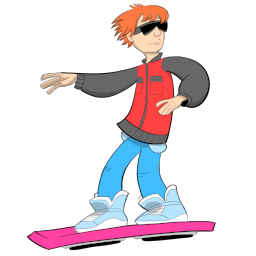
\includegraphics[width=1in]{images/HoverBoard-small.png}
	\end{wrapfigure}

	We denote the restriction on the hover board's movement by the vector
	$\mat{3 \\1}$. By this we mean that if
	the hover board traveled ``forward'' for one hour, it would move along a
	``diagonal'' path that would result in a displacement of 3 km East and
	1 km North of its starting location.
\end{minipage}

\begin{minipage}{\linewidth}
	\vspace{.5cm}
	\begin{wrapfigure}{l}{1in}
	\vspace{-.8cm}
	
\includegraphics[width=1in]{images/MagicCarpet-small.png}
	\end{wrapfigure}

	We denote the restriction on the magic carpet's movement by the vector
	$\mat{1 \\2 }$. By this we mean that if the
	magic carpet traveled ``forward'' for one hour, it would move along a
	``diagonal'' path that would result in a displacement of 1 km East and
	2 km North of its starting location.
\end{minipage}

\lfoot{\footnotesize Drawings by \url{@DavidsonJohnR} (twitter)}

\vspace{10mm}
\end{slide}

\begin{slide}
% Scenario Section
\textbf{Scenario One: The Maiden Voyage}

Your Uncle Cramer suggests that your first adventure should be to go visit
the wise man, Old Man Gauss. Uncle Cramer tells you that Old Man Gauss
lives in a cabin that is 107 km East and 64 km North of your home.

\vspace{5mm}

\textbf{Task:}
\par
Investigate whether or not you can use the hover board and the magic
carpet to get to Gauss's cabin. If so, how? If it is not possible to
get to the cabin with these modes of transportation, why is that the case?

%\vspace{5mm}
% As a group, state and explain your answer(s) on the group whiteboard. Use
% the vector notation for each mode of transportation as part of your
% explanation and use a diagram or graphic to help illustrate your
% point(s).
\end{slide}
\end{iola}

\section*{Sets and Set Notation}
\vspace{-.5cm}

\begin{slide}[+1]
	\SavedDefinitionRender{Set}

	\begin{definition}
		\raggedright
		Some common sets are
		\begin{itemize}
			\item[] $\N=\Set{\text{natural numbers}} = \Set{\text{non-negative whole numbers}}$.
			\item[] $\Z=\Set{\text{integers}} = \Set{\text{whole numbers, including negatives}}$.
			\item[] $\R=\Set{\text{real numbers}}$.
			\item[] $\R^n=\Set{\text{vectors in $n$-dimensional Euclidean space}}$.
		\end{itemize}
	\end{definition}
\end{slide}
\begin{slide}
	\question
	\begin{parts}
		\item Which of the following statements are true?
		\begin{enumerate}
			\item $3\in\Set{1,2,3}$.
				\begin{solution}[inline]True\end{solution}
			\item $1.5\in\Set{1,2,3}$.
				\begin{solution}[inline]False\end{solution}
			\item $4\in\Set{1,2,3}$.
				\begin{solution}[inline]False\end{solution}
			\item ``b''$\in \Set{ x \given x\text{ is an English letter}}$.
				\begin{solution}[inline]True\end{solution}
			\item ``\`o''$\in \Set{x \given x\text{ is an English letter}}$.
				\begin{solution}[inline]False\end{solution}
			\item $\Set{1,2} \subseteq \Set{1,2,3}$.
				\begin{solution}[inline]True\end{solution}
			\item For some $a\in \Set{1,2,3}$, $a \geq 3$.
				\begin{solution}[inline]True\end{solution}
			\item For any $a\in \Set{1,2,3}$, $a\geq 3$.
				\begin{solution}[inline]False\end{solution}
			\item $1 \subseteq \Set{1,2,3}$.
				\begin{solution}[inline]False\end{solution}
			\item $\Set{1,2,3}=\Set{x\in\R \given 1\leq x\leq 3}$.
				\begin{solution}[inline]False\end{solution}
			\item $\Set{1,2,3}=\Set{x\in\Z \given 1\leq x\leq 3}$.
				\begin{solution}[inline]True\end{solution}
		\end{enumerate}
	\end{parts}
\end{slide}

\begin{slide}
	\bookonlynewpage
	\question
	\begin{annotation}
		\begin{goals}
			\Goal{Practice writing sets using set-builder notation.}

			The goal of this problem is to
			\begin{itemize}
				\item Express English descriptions using math notation.
				\item Recognize there is more than one correct way to
					write formal math.
				\item Preview vector form of a line.
			\end{itemize}
		\end{goals}

		\begin{notes}
			\begin{itemize}
				\item There are multiple correct ways to write
					each of these sets. It's a good opportunity
					to get many correct and incorrect sets up on the
					board for discussing.
				\item Don't worry about the geometry of $B$. That's coming
					in a later problem.
			\end{itemize}
		\end{notes}
	\end{annotation}
		Write the following in set-builder notation
	\begin{parts}
			\item The subset $A\subseteq \R$ of real numbers larger than $\sqrt{2}$.
				\begin{solution}
					$\Set*{x\in\R \given x>\sqrt{2}}$.
				\end{solution}
			\item The subset $B\subseteq \R^2$ of vectors whose first coordinate
			is twice the second.
				\begin{solution}
					$\Set*{\vec v\in\R^2\given \vec v=\mat{a\\b}\text{ with }a=2b}$
					or
					$\Set*{\vec v\in\R^2\given\vec v=\mat{2t\\t}\text{ for some }t\in \R}$\\
					or
					$\Set*{\mat{a\\b}\in\R^2\given a=2b}$.
				\end{solution}
	\end{parts}
\end{slide}

\begin{slide}
	\displayonlynewpage
	\begin{bookonly}\vspace{\stretch{1}}\end{bookonly}
	\SavedDefinitionRender{UnionsIntersections}

	\question
	\begin{annotation}
		\begin{goals}
			\Goal{Apply the definition of $\cup$ and $\cap$.}
		\end{goals}

		\begin{notes}
			\begin{itemize}
				\item It's not important to emphasize that $\cup$ and $\cap$ are binary
			operations but we ask for $X\cup Y\cup Z$ without parenthesis.
			Students won't worry if you don't bring it up.
				\item It won't be clear to them how to write the empty set.
					Some will write $\{\emptyset\}$. Make sure this comes out.
			\end{itemize}
		\end{notes}
	\end{annotation}
	Let $X=\Set{1,2,3}$ and $Y=\Set{2,3,4,5}$ and $Z=\Set{4,5,6}$.  Compute
	\begin{parts}
		\item $X\cup Y$ \begin{solution}[inline]$\Set{1,2,3,4,5}$\end{solution}
		\item $X\cap Y$ \begin{solution}[inline]$\Set{2,3}$\end{solution}
		\item $X\cup Y\cup Z$ \begin{solution}[inline]$\Set{1,2,3,4,5,6}$\end{solution}
		\item $X\cap Y\cap Z$ \begin{solution}[inline]$\emptyset=\Set{}$\end{solution}
	\end{parts}
	\begin{bookonly}\vspace{\stretch{1}}\end{bookonly}
\end{slide}








\begin{lesson}
	\Title{Visualizing Sets, Formal Language of Linear Combinations}

	\Heading{Textbook}
	Module 1

	\Heading{Objectives}
	\begin{itemize}
		\item Draw pictures of formally-described subsets of $\R^2$.
		\item Graphically represent $\cup$ and $\cap$ for subsets of $\R^2$.
		\item Graphically represent linear combinations and then come up with
			algebraic arguments to support graphical intuition.
	\end{itemize}

	\Heading{Motivation}

	We want to build a bridge between the formal language of linear combinations
	and set-builder notation and geometric intuition. Where as last time
	the focus was on formal language, this time the focus is on linking geometry
	to formal descriptions.


\end{lesson}

\begin{slide}
	\bookonlynewpage
	\question
	\begin{annotation}
		\begin{goals}
			\Goal{Visualize sets of vectors.}

			The goal of this problem is to
			\begin{itemize}
				\item Apply set-builder notation in the context of vectors.
				\item Distinguish between ``for all'' and ``for some''
					in set builder notation.
				\item Practice unions and intersections.
				\item Practice thinking about set equality.
			\end{itemize}
		\end{goals}

		\begin{notes}
			\begin{itemize}
				\item 1--3 will be easy.
				\item Have a discussion about when you
					should draw vectors as arrows
					vs\mbox{.} as points.
				\item 4 gets at a subtle point that will come up again
					when we define span.
				\item Many will miss 7. Writing a proof for this is
					good practice.
			\end{itemize}
		\end{notes}
	\end{annotation}
	Draw the following subsets of $\R^2$.
	\begin{parts}
		\item $V=\Set*{\vec x\in\R^2 \given \vec x=\mat{0\\t}\text{ for some }t\in\R}$.
		\item $H=\Set*{\vec x\in\R^2 \given \vec x=\mat{t\\0}\text{ for some }t\in\R}$.
		\item $D=\Set*{\vec x\in\R^2 \given \vec x=t\mat{1\\1}\text{ for some }t\in\R}$.
		\begin{solution}
	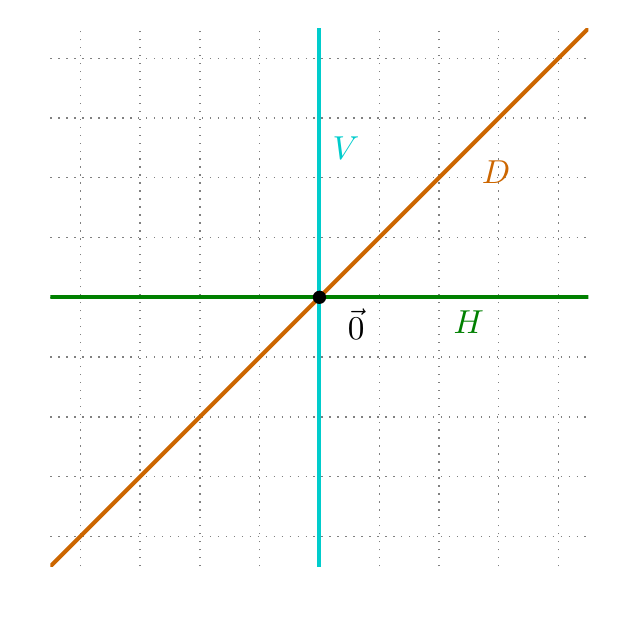
\begin{tikzpicture}[scale=1.2, >=latex]
    \begin{axis}[scale=1,
		    axis equal image,
		    axis line style={draw=none},
		    tick style={draw=none},
		    yticklabels={,,},
		    xticklabels={,,},
		 xmin=-4.5,
		 xmax=4.5,
		 ymin=-4.5,
		 ymax=4.5,
		 major grid style={dotted, gray},
                 xtick={-10,-9,...,10},
                 ytick={-10,-9,...,10},
                 grid=both,
		 anchor=origin]

	    \draw[Green, very thick] (-5,0) -- (5,0) node[near end, below] {$H$};
	    \draw[cyan!80!black, very thick] (0,-5) -- (0,5) node[near end, right] {$V$};
	    \draw[orange!80!black, very thick] (-5,-5) -- (5,5) node[near end, below right] {$D$};

	    \fill[fill=black] (0,0) circle[radius=2pt] node[below right, xshift=5pt] {\color{black}$\vec 0$};
    \end{axis}
\end{tikzpicture}
		\end{solution}
		\item $N=\Set*{\vec x\in\R^2 \given \vec x=t\mat{1\\1}\text{ for all }t\in\R}$.
				\begin{solution}[inline]
			$N=\Set{}$.
		\end{solution}

		\item $V\cup H$.
			\begin{solution}[inline]
			$V\cup H$ looks like a ``$+$'' going through the origin.
		\end{solution}
		\item $V\cap H$.
			\begin{solution}[inline]
				$V\cap H=\Set{\vec 0}$ is just the origin.
		\end{solution}
		\item Does $V\cup H=\R^2$?
			\begin{solution}
				No. $V\cup H$ does not contain $\mat{1\\1}$ while $\R^2$ does contain
				$\mat{1\\1}$.
			\end{solution}
	\end{parts}
\end{slide}


	\begin{bookonly}\begin{center}\hspace{-2cm}\triplegrid\hspace{-2cm}\triplegrid\end{center}\end{bookonly}
	\bookonlynewpage
	\displayonlynewpage
\section*{Vector Combinations}
	\vspace{-1em}

\begin{slide}
	\SavedDefinitionRender{LinearCombination}

	\question
	\label{ProbSkewBasis}
	\begin{annotation}
		\begin{goals}
			\Goal{Practice linear combinations.}

			The goal of this problem is to
			\begin{itemize}
				\item Practice using the formal term \emph{linear combination}.
				\item Foreshadow span.
			\end{itemize}
		\end{goals}

		\begin{notes}
			\begin{itemize}
				\item In 2, the question should arise: ``Is $3\vec v_1$
					a linear combination of $\vec v_1$ \emph{and}
					$\vec v_2$?'' Address this.
				\item Refer to the magic carpet ride for 5. You don't
					need to do a full proof.
			\end{itemize}
		\end{notes}
	\end{annotation}
	Let $\vec v_1=\mat{1\\1}$, $\vec v_2=\mat{1\\-1}$, and $\vec w=2\vec v_1+\vec v_2$.
	\begin{parts}
		\item Write $\vec w$ as a column vector. When $\vec w$ is written as a
			linear combination of $\vec v_1$ and $\vec v_2$, what are the
			coefficients of $\vec v_1$ and $\vec v_2$?
			\begin{solution}
				$\vec w=\mat{3\\1}$; the coefficients are $(2,1)$.
			\end{solution}
		\item Is $\mat{3\\3}$ a linear combination of $\vec v_1$ and $\vec v_2$?
			\begin{solution}[inline]
				Yes. $\mat{3\\3}=3\vec v_1+0\vec v_2$.
			\end{solution}

		\item Is $\mat{0\\0}$ a linear combination of $\vec v_1$ and $\vec v_2$?
			\begin{solution}[inline]
				Yes. $\vec 0=0\vec v_1+0\vec v_2$.
			\end{solution}
		\item Is $\mat{4\\0}$ a linear combination of $\vec v_1$ and $\vec v_2$?
			\begin{solution}[inline]
				Yes. $\mat{4\\0}=2\vec v_1+2\vec v_2$.
			\end{solution}
		\item Can you find a vector in $\R^2$ that isn't a linear combination of
		$\vec v_1$ and $\vec v_2$?
			\begin{solution}
				No. $\mat{1\\0}=\tfrac{1}{2}\vec v_1+\tfrac{1}{2}\vec v_2$ and
				$\mat{0\\1}=\tfrac{1}{2}\vec v_1-\tfrac{1}{2}\vec v_2$.
				Therefore
				\[
					\mat{a\\b}
					= a\mat{1\\0}+b\mat{0\\1}
					= a(\tfrac{1}{2}\vec v_1+\tfrac{1}{2}\vec v_2)
						+b(\tfrac{1}{2}\vec v_1-\tfrac{1}{2}\vec v_2)
					=(\tfrac{a+b}{2})\vec v_1+(\tfrac{a-b}{2})\vec v_2.
				\]
				Therefore any vector in $\R^2$ can be written as linear combinations
				of $\vec v_1$ and $\vec v_2$.
			\end{solution}
		\item Can you find a vector in $\R^2$ that isn't a linear combination of
			$\vec v_1$?
			\begin{solution}
				Yes. All linear combinations of $\vec v_1$ have equal $x$ and
				$y$ coordinates, therefore $\vec w=\mat{2\\1}$ is not a linear
				combination of $\vec v_1$.
			\end{solution}
	\end{parts}
\end{slide}

\begin{slide}
	\bookonlynewpage
	\question
	\begin{annotation}
		\begin{goals}
			\Goal{Practice formal writing.}
		\end{goals}

		\begin{notes}
			\begin{itemize}
				\item Make everyone \emph{write}. They will think
					they can do it, but they will find it hard if
					they try.
			\end{itemize}
		\end{notes}
	\end{annotation}
	Recall the \emph{Magic Carpet Ride} task where the hover board could
	travel in the direction $\vec h=\mat{3\\1}$ and the magic carpet could
	move in the direction $\vec m=\mat{1\\2}$.
	\begin{parts}
		\item Rephrase the sentence \emph{``Gauss can be reached using just the
			magic carpet and the hover board''} using formal mathematical
			language.
			\begin{solution}
				Gauss's location can be written as a linear combination of
				$\vec m$ and $\vec h$.
			\end{solution}
		\item Rephrase the sentence \emph{``There is nowhere Gauss can hide
			where he is inaccessible by magic carpet and hover board''} using
			formal mathematical language.
			\begin{solution}
				Every vector in $\R^2$ can be written as a linear combination
				of $\vec m$ and	$\vec h$.
			\end{solution}
		\item Rephrase the sentence \emph{``$\R^2$ is the set of all linear
			combinations of $\vec h$ and $\vec m$''} using formal mathematical
			language.
			\begin{solution}
				$\R^2=\Set{\vec v\given \vec v=t\vec m+s\vec h\text{ for some }t,s\in \R}$.
			\end{solution}
	\end{parts}
\end{slide}
\begin{slide}
	\question
	Hi
	\question
	There

\end{slide}

\end{document}
